\section{Simulation studies}\label{sec:simulation}

We use simulation to answer five questions that the application raises but
cannot settle on its own:
(S0) whether the finite-volume SPDE and the empirical Bayes Laplace
approximation recover the field and give calibrated intervals;
(S1) whether residual spatial structure left by a boosting model can be
detected and modelled, and whether modelling it improves forecasts;
(S2) how national indicators behave under spatial confounding;
(S3) whether state dependence can be separated from persistent heterogeneity;
(S4) whether biome-specific climate effects are recovered better by spatially
varying coefficients than by SHAP summaries.
All code is in the supplementary material.

\subsection{Data-generating process}\label{sec:sim-dgp}

The simulator mimics the structure of the ACLED grid. The domain is a
$40 \times 30$ block of $0.5^\circ$ cells between $10^\circ$E and $30^\circ$E and
between $5^\circ$S and $10^\circ$N (1{,}200 cells of about 55\,km), with 104
training weeks, 52 test weeks and 12 burn-in weeks. Countries are the Voronoi
cells of randomly placed seeds (14 countries; 25 in S2). Four biomes are
latitude bands with boundaries perturbed by a smooth random field, ordered from
``cold'' (biome 1) to ``tropical'' (biome 4). Population is a standardised
Mat\'ern field (range 250\,km) plus white noise. Temperature and precipitation
anomalies are standardised AR(1) processes in time (coefficients 0.6 and 0.3) of
Mat\'ern fields with ranges of 800 and 500\,km. Three national covariates
$Z_0, Z_1, Z_2$ are standard normal across countries; $Z_1$ and $Z_2$ have no
effect but, like the national indicators in the data, allow trees to identify
countries. Outcomes are generated sequentially from
\begin{equation}\label{eq:sim}
\logit\pi_{st} = \beta_0 + \beta_{\mathrm{pop}}\mathrm{pop}_s
+ \delta\log\Bigl(1 + \textstyle\sum_{l=1}^{4} y_{s,t-l}\Bigr)
+ \beta(s)\,\mathrm{temp}_{st} + \beta_{\mathrm{prec}}\mathrm{prec}_{st}
+ \alpha Z_{0,c(s)} + u_{c(s)} + w(s) + v(s,t),
\end{equation}
with $\beta(s) = \gamma_{b(s)} + \eta(s)$, $u_c \sim \Normal(0, 0.3^2)$, and
$w$, $\eta$ and $v$ drawn from the GMRFs of Section~\ref{sec:methods}. Unless
stated otherwise, $\beta_0 = -4$, $\beta_{\mathrm{pop}} = 0.5$, $\delta = 0.6$,
$\bgamma = (-0.3, -0.1, 0.1, 0.3)$, $\eta \equiv 0$, $\beta_{\mathrm{prec}} = -0.15$,
$\alpha = 0$, $\sigma_w = 1$, $\rho_w = 400$\,km and $v \equiv 0$. The resulting
prevalence of event weeks is 3--4\%, close to that of the data. Spatial
confounding (S2) is induced by setting
$Z_{0,c} = \varrho\,\tilde\ell_c + (1-\varrho^2)^{1/2}\epsilon_c$, where
$\tilde\ell_c$ is the standardised country average of $u_c + w(s)$ and
$\epsilon_c \sim \Normal(0,1)$.

The boosting model is XGBoost with the hyperparameters of the original analysis \citep{menicali2026conflicts}
(depth 5, learning rate 0.05, row and column subsampling 0.8, minimum child
weight 30, $L_2$ penalty 5; 300 rounds), without class weights. Its features
are population, distance from the equator, biome, the two anomalies, $Z_0$--$Z_2$
and the four-week event count. As in the original analysis, the features
include no coordinates.

\subsection{S0: accuracy of the field representation and of the Laplace engine}\label{sec:sim-engine}

We simulate $w$ from the lattice SPDE~\eqref{eq:Qs} on the $40 \times 30$ domain
with $\rho_w = 400$\,km and $\sigma_w = 1$, and Bernoulli outcomes for 40 weeks
from $\logit\pi_{st} = -2 + 0.5\,x_{st} + w(s)$ with $x_{st} \sim \Normal(0,1)$,
50 replicates. Table~\ref{tab:s0} summarises the results. Across 2{,}000
draws, the empirical marginal variance of the field is 1.07 in cells at least
eight cells (about 440\,km) from the edge of the domain, against a nominal 1.
At the edge it is 2.02, the doubling induced by the Neumann boundary that
motivates the buffer of Remark~\ref{rem:boundary}. The hyperparameters are
recovered with little bias ($\hat\rho_w = 399$\,km, $\hat\sigma_w = 0.99$),
and the posterior mean of $w$ has correlation 0.96 with the truth. Plug-in 95\%
intervals cover $0.5$ in 92\% of replicates (Monte Carlo SE 3.8\%) and cover
$-2 + w(s)$ for 94.4\% of cells, so ignoring the uncertainty in $\btheta$ costs
little here. A fit takes about 5 seconds on one core.

\begin{table}
\caption{S0: accuracy of the finite-volume SPDE field and of the empirical
Bayes Laplace approximation (50 replicates).}\label{tab:s0}
\centering\small
\begin{tabular}{@{}lcc@{}}
\toprule
Quantity & common ($b_0=-2$, 50 reps) & rare ($b_0=-4.5$, 50 reps) \\
\midrule
Prevalence of event weeks & 0.161 (0.030) & 0.019 (0.005) \\
$\hat\rho_w$ (km) [truth 400] & 420 (40) & 409 (51) \\
$\hat\sigma_w$ [truth 1] & 0.884 (0.064) & 0.875 (0.075) \\
$\hat b_1$ [truth 0.5] & 0.494 (0.016) & 0.502 (0.021) \\
Coverage of 95\% interval for $b_1$ & 0.88 (0.05) & 0.96 (0.03) \\
Coverage of 95\% intervals for $b_0 + w(s)$ (share of cells) & 0.948 (0.009) & 0.943 (0.017) \\
$\mathrm{cor}(\hat w, w)$ & 0.954 (0.008) & 0.914 (0.018) \\
Fit time (s) & 2.4 (0.7) & 3.4 (0.8) \\
Marginal variance of $w$, interior cells [nominal 1] & 1.07 & -- \\
Marginal variance of $w$, edge cells & 2.02 & -- \\
\bottomrule
\end{tabular}

\end{table}

\subsection{S1: residual structure after boosting}\label{sec:sim-residual}

Data are generated from \eqref{eq:sim} with the default parameters, and the
models are trained on the first 104 weeks and evaluated on the following 52,
as in the original analysis. Table~\ref{tab:s1} reports
out-of-sample scores over 20 replicates and Table~\ref{tab:s1-field} the
residual diagnostics and the recovery of the field. Figure~\ref{fig:s1} shows
one replicate.

Three findings stand out. First, boosting does not absorb the residual field
even with in-sample training on the same locations. Moran's $I$ of the cell
residuals of the XGBoost model as used in the original analysis is 0.33
(SD 0.07 across replicates), against an expected value of about $-0.001$ under
independence. For spatially cross-fitted XGBoost it is 0.59. The trees recover
part of the field through country-identifying national covariates, which is
exactly the leakage that makes in-sample residuals understate the
spatial structure (Section~\ref{sec:methods-hybrid}). Second, the field
estimated on top of the cross-fitted offset recovers the truth well
(correlation between $\hat w$ and $w$ of 0.81 when $u$ is included), and its hyperparameters are close to
the truth: $\hat\rho_w = 373$\,km against 400 and $\hat\sigma_w = 0.94$
against 1. Third, modelling the residual field improves forecasts for the
same places. The hybrid model improves on the original XGBoost in log score
in all 20 replicates (mean difference $-0.0031$, SE $0.0003$) and in AUC-PR in 19
of 20 (mean difference $+0.011$, SE $0.001$). The correctly specified parametric
model is better still, in every replicate. The persistence baseline reaches an
AUC-PR of 0.10, against 0.27 for the true probabilities; in these simulations
persistence is a much weaker benchmark than it is likely to be in the data,
where some cells record events almost every week.

\begin{table}
\caption{S1: out-of-sample scores on the 52 test weeks (mean over 20
replicates, Monte Carlo standard error in parentheses). Lower is better for
the log and Brier scores.}\label{tab:s1}
\centering\small
\begin{tabular}{@{}lcccc@{}}
\toprule
Model & Log score & Brier & AUC-PR & AUC-ROC \\
\midrule
True probabilities & 0.1429 (0.0080) & 0.0367 (0.0026) & 0.267 (0.018) & 0.826 (0.005) \\
XGBoost (as in original analysis) & 0.1501 (0.0084) & 0.0377 (0.0027) & 0.235 (0.017) & 0.790 (0.006) \\
XGBoost, spatially cross-fitted & 0.1649 (0.0098) & 0.0402 (0.0031) & 0.152 (0.015) & 0.715 (0.008) \\
Cross-fitted XGBoost + $w$ & 0.1470 (0.0082) & 0.0374 (0.0027) & 0.245 (0.017) & 0.809 (0.005) \\
Cross-fitted XGBoost + $u + w$ & 0.1469 (0.0082) & 0.0374 (0.0027) & 0.245 (0.017) & 0.810 (0.005) \\
Parametric model with $u + w$ & 0.1457 (0.0081) & 0.0371 (0.0026) & 0.253 (0.018) & 0.814 (0.005) \\
Persistence baseline & -- & -- & 0.103 (0.009) & -- \\
\bottomrule
\end{tabular}

\end{table}

\begin{table}
\caption{S1: residual diagnostics and recovery of the field (mean and SD over
20 replicates).}\label{tab:s1-field}
\centering\small
\begin{tabular}{@{}lcc@{}}
\toprule
Quantity & Mean & SD \\
\midrule
Moran's $I$ of cell residuals, XGBoost (original) & 0.330 & 0.069 \\
Moran's $I$ of cell residuals, XGBoost cross-fitted & 0.591 & 0.064 \\
$\mathrm{cor}(\hat w, w)$, XGBoost + $w$ & 0.768 & 0.049 \\
$\mathrm{cor}(\hat w, w)$, XGBoost + $u + w$ & 0.814 & 0.036 \\
$\hat\rho_w$ (km), XGBoost + $u + w$ [truth 400] & 373.374 & 48.288 \\
$\hat\sigma_w$, XGBoost + $u + w$ [truth 1] & 0.943 & 0.095 \\
\bottomrule
\end{tabular}

\end{table}

\begin{figure}
\centering
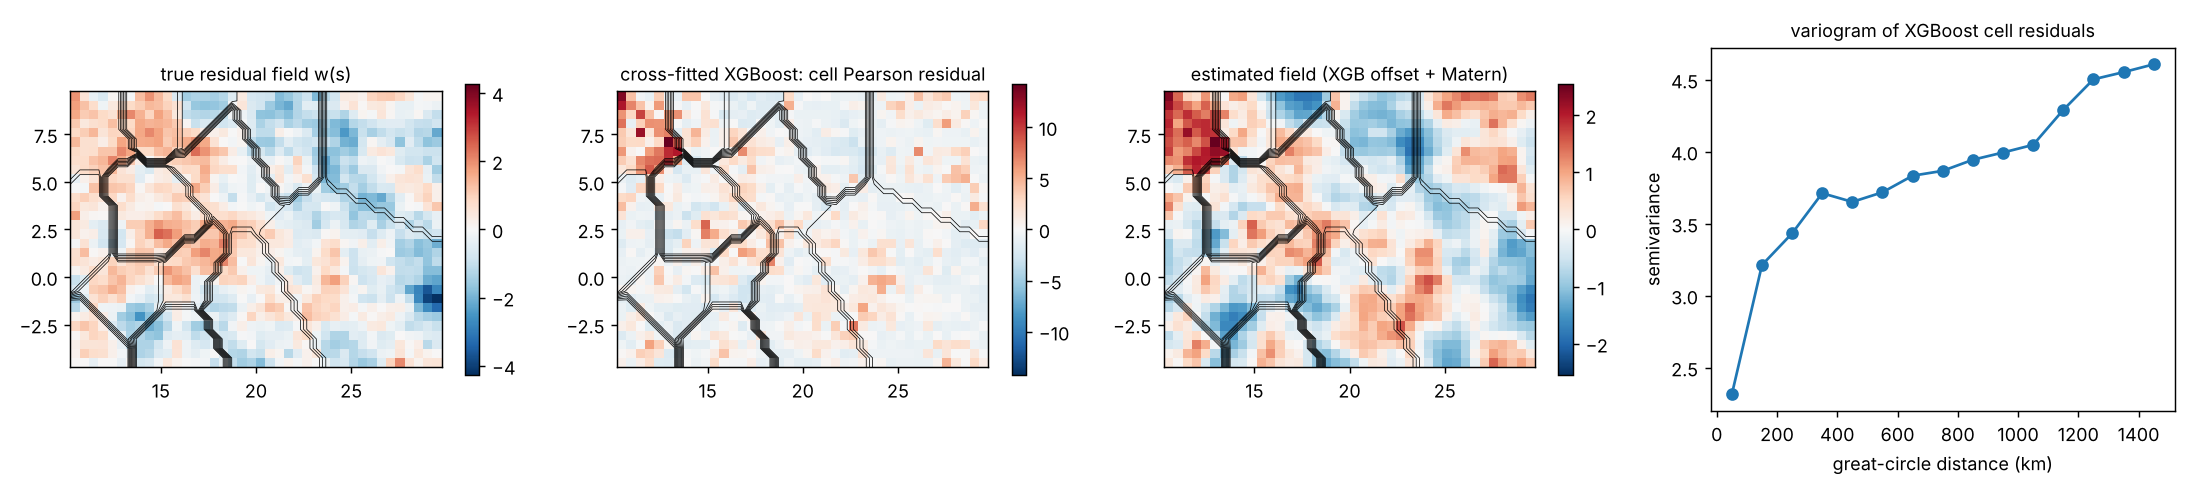
\includegraphics[width=\textwidth]{figures/s1_maps.png}
\caption{S1, one replicate. From left: the true field $w$; standardised cell
residuals of the cross-fitted XGBoost model; posterior mean of $w$ in the
hybrid model~\eqref{eq:hybrid}; semivariogram of the XGBoost cell residuals.
Lines are country borders.}\label{fig:s1}
\end{figure}

\subsection{S2: national indicators under spatial confounding}\label{sec:sim-confounding}

Three scenarios with 25 countries and 30 replicates each are considered:
no confounding with $\alpha = 0$ ($\varrho = 0$); confounding with $\alpha = 0$
($\varrho = 0.8$); and confounding with a true effect $\alpha = -0.3$. We
compare the estimators of Section~\ref{sec:methods-confounding} with the
XGBoost summary of the original analysis. For the latter, the effect of $Z_0$
is summarised by the least-squares slope of its SHAP values on $Z_0$, with
intervals from 20 replicates of the $5^\circ$ block bootstrap on a fixed 30\%
subsample of the training data, as in the original analysis.

\begin{table}
\caption{S2: estimation of the effect $\alpha$ of a national indicator (30
replicates per scenario). Coverage of nominal 95\% intervals and the
proportion of replicates in which the interval excludes zero.
$^\dagger$Least-squares slope of SHAP values on $Z_0$; 95\% block-bootstrap
percentile interval.}\label{tab:s2}
\centering\small
\begin{tabular}{@{}lccccc@{}}
\toprule
Estimator & Mean & Emp.\ SD & Mean SE & Coverage & Reject $\alpha=0$ \\
\midrule
\multicolumn{6}{@{}l}{\emph{No confounding, $\alpha = 0$}} \\
\quad Logistic regression & -0.013 & 0.102 & 0.016 & 0.27 & 0.73 \\
\quad + country effects $u$ & -0.002 & 0.124 & 0.132 & 0.97 & 0.03 \\
\quad + spatial field $w$ & 0.002 & 0.068 & 0.055 & 0.90 & 0.10 \\
\quad + $u$ + $w$ & -0.002 & 0.070 & 0.084 & 1.00 & 0.00 \\
\quad spatial+ with $u$ + $w$ & -0.002 & 0.077 & 0.085 & 1.00 & 0.00 \\
\quad XGBoost SHAP slope$^\dagger$ & 0.002 & 0.088 & 0.070 & 0.60 & 0.40 \\
\multicolumn{6}{@{}l}{\emph{Confounding, $\alpha = 0$}} \\
\quad Logistic regression & 0.469 & 0.095 & 0.017 & 0.00 & 1.00 \\
\quad + country effects $u$ & 0.517 & 0.115 & 0.086 & 0.00 & 1.00 \\
\quad + spatial field $w$ & 0.197 & 0.072 & 0.060 & 0.13 & 0.87 \\
\quad + $u$ + $w$ & 0.204 & 0.059 & 0.081 & 0.20 & 0.80 \\
\quad spatial+ with $u$ + $w$ & 0.151 & 0.065 & 0.084 & 0.50 & 0.50 \\
\quad XGBoost SHAP slope$^\dagger$ & 0.394 & 0.093 & 0.086 & 0.00 & 1.00 \\
\multicolumn{6}{@{}l}{\emph{Confounding, $\alpha = -0.3$}} \\
\quad Logistic regression & 0.250 & 0.102 & 0.017 & 0.00 & 1.00 \\
\quad + country effects $u$ & 0.269 & 0.117 & 0.085 & 0.00 & 0.77 \\
\quad + spatial field $w$ & -0.091 & 0.074 & 0.060 & 0.17 & 0.33 \\
\quad + $u$ + $w$ & -0.086 & 0.059 & 0.082 & 0.17 & 0.20 \\
\quad spatial+ with $u$ + $w$ & -0.133 & 0.059 & 0.084 & 0.40 & 0.23 \\
\quad XGBoost SHAP slope$^\dagger$ & 0.178 & 0.093 & 0.075 & 0.00 & 0.70 \\
\bottomrule
\end{tabular}

\end{table}

Table~\ref{tab:s2} reports the results. Without confounding, all estimators
are centred on zero, but intervals that ignore the country-level structure of
the covariate are badly anticonservative. Logistic regression reports a
standard error of 0.017 against an empirical SD of 0.10, so it covers in 27\%
of replicates and declares a non-existent effect significant in 73\%. Country
effects alone restore nominal coverage. The block-bootstrap summary of the
original analysis does little better than logistic regression: its 95\%
interval excludes zero in 40\% of replicates and its interquartile range, the
criterion used in the original analysis, in 70\%, although $Z_0$ has no effect.
The reason is that $5^\circ$ blocks do not resample countries, the units at
which $Z_0$ varies.

Under confounding with $\alpha = 0$, no estimator is unbiased. Logistic
regression and the country-effects model report $\hat\alpha \approx 0.47$--$0.52$
and always reject. The spatial field removes about 60\% of the bias
($\hat\alpha \approx 0.20$), and spatial+ removes about 70\% ($0.15$; coverage 0.50).
XGBoost reports a SHAP slope of 0.39, with an interquartile range that excludes
zero in every replicate. With a true protective effect ($\alpha = -0.3$), the
naive estimators and XGBoost report effects of the \emph{wrong sign}
($+0.25$ and $+0.18$, the latter with an interquartile range excluding zero in
90\% of replicates). The spatial estimators recover the sign but only a third
to a half of the magnitude ($-0.09$ to $-0.13$). The lesson for the national
sustainability indicators is that the data can reveal whether an association
survives spatial adjustment, but not its causal size. A large SHAP contribution
of a national indicator, stable across block-bootstrap replicates, is fully
compatible with no effect at all.

\subsection{S3: state dependence versus persistent heterogeneity}\label{sec:sim-persistence}

Two data-generating processes on a smaller $16 \times 14$ domain
(224 cells, 6 countries, 104 training weeks, 20 replicates each) produce
similar autocorrelation in $Y_{st}$ for different reasons:
\emph{state dependence} with $\delta = 1$ and a weak field ($\sigma_w = 0.3$), and
\emph{heterogeneity} with no state dependence ($\delta = 0$) but a strong
static field ($\sigma_w = 1.3$) and a space-time AR(1) field
($\sigma_v = 0.7$, $\phi = 0.9$ per week, $\rho_v = 300$\,km). We fit
model~\eqref{eq:model} with lags only, with lags and $w$, and with lags, $w$
and $v$, where $v$ is resolved at four-week steps. We also report the share
of total mean absolute SHAP value that XGBoost assigns to the lag feature.
Results are in Table~\ref{tab:s3}.

Under state dependence, ignoring the latent field inflates $\hat\delta$ by about
a third (1.32; coverage 0.35). Both latent specifications are approximately
unbiased (1.02 and 0.98) and have nominal coverage. Under heterogeneity the
contrast is much sharper. With lags only, $\hat\delta = 2.13$ although the true
value is zero, and adding the static field halves the bias to 0.70 without
restoring coverage: slowly varying episodes act as state dependence. Only the
model with the space-time field brings the estimate close to zero (0.11, with
an empirical SD of 0.12 and a coverage of 0.80). The remaining bias reflects the
approximation of a weekly AR(1) process by a field resolved at four-week steps.
In the application, the temporal resolution of $v$ should therefore be chosen
by marginal likelihood. Finally, the XGBoost importance of the lag feature is
\emph{larger} under heterogeneity (share 0.17) than under state dependence (0.11).
Variable importance of recent history therefore says nothing about whether
violence begets violence.

\begin{table}
\caption{S3: estimation of the state-dependence parameter $\delta$ (20
replicates per scenario), and the share of the XGBoost mean absolute SHAP
value assigned to the lag feature.}\label{tab:s3}
\centering\small
\begin{tabular}{@{}lcccc@{}}
\toprule
Estimator & Mean $\hat\delta$ & Emp.\ SD & Mean SE & Coverage \\
\midrule
\multicolumn{5}{@{}l}{\emph{State dependence ($\delta = 1$)}} \\
\quad Lags only & 1.263 & 0.107 & 0.136 & 0.60 \\
\quad Lags + $w$ & 1.032 & 0.131 & 0.139 & 0.90 \\
\quad Lags + $w$ + $v$ (4-week steps) & 0.990 & 0.135 & 0.140 & 0.95 \\
\quad Lags + $w$ + $v$ (weekly steps) & 0.997 & 0.143 & 0.140 & 0.95 \\
\quad XGBoost: share of mean $|$SHAP$|$ for lags & 0.108 & 0.034 & -- & -- \\
\multicolumn{5}{@{}l}{\emph{Heterogeneity ($\delta = 0$)}} \\
\quad Lags only & 1.614 & 0.386 & 0.099 & 0.00 \\
\quad Lags + $w$ & 0.464 & 0.093 & 0.111 & 0.00 \\
\quad Lags + $w$ + $v$ (4-week steps) & 0.045 & 0.152 & 0.119 & 0.90 \\
\quad Lags + $w$ + $v$ (weekly steps) & 0.011 & 0.162 & 0.120 & 0.90 \\
\quad XGBoost: share of mean $|$SHAP$|$ for lags & 0.094 & 0.038 & -- & -- \\
\multicolumn{5}{@{}l}{\emph{Mixed ($\delta = 0.5$)}} \\
\quad Lags only & 1.659 & 0.351 & 0.106 & 0.00 \\
\quad Lags + $w$ & 0.782 & 0.111 & 0.115 & 0.25 \\
\quad Lags + $w$ + $v$ (4-week steps) & 0.545 & 0.152 & 0.120 & 0.85 \\
\quad Lags + $w$ + $v$ (weekly steps) & 0.535 & 0.172 & 0.120 & 0.80 \\
\quad XGBoost: share of mean $|$SHAP$|$ for lags & 0.116 & 0.044 & -- & -- \\
\bottomrule
\end{tabular}

\end{table}

\subsection{S4: biome-specific climate effects}\label{sec:sim-svc}

The temperature effect follows \eqref{eq:svc}, with biome means
$\bgamma = (-0.3, -0.1, 0.1, 0.3)$ and a within-biome Mat\'ern deviation $\eta$
($\sigma_\eta = 0.15$, $\rho_\eta = 600$\,km); $\sigma_w = 0.8$ and 30
replicates. We compare fixed biome-specific slopes without and with $u + w$,
the SVC model~\eqref{eq:svc}, the per-biome least-squares slope of the XGBoost
SHAP values, and the statistic of the original analysis, the median SHAP value
within each biome, with the interquartile range over 10 block-bootstrap
replicates. Coverage is reported for both the biome mean $\gamma_b$ and the
realised biome-average effect $\bar\beta_b$ (Section~\ref{sec:methods-svc}).

\begin{table}
\caption{S4: estimation of biome-specific temperature effects (30
replicates). ``Detects sign'': proportion of replicates in which the interval
excludes zero on the correct side. $^\ddagger$Median SHAP value within the biome
with the interquartile range of the bootstrap replicates, as in the original
analysis; it estimates neither $\gamma_b$ nor $\bar\beta_b$.}\label{tab:s4}
\centering\small
\begin{tabular}{@{}lcccc@{}}
\toprule
Estimator / biome & Mean est. & Cov.\ $\gamma_b$ & Cov.\ $\bar\beta_b$ & Detects sign \\
\midrule
\multicolumn{5}{@{}l}{\emph{Biome slopes, no latent effects}} \\
\quad biome 1 ($\gamma = -0.3$) & -0.273 & 0.57 & 0.77 & 1.00 \\
\quad biome 2 ($\gamma = -0.1$) & -0.083 & 0.57 & 0.83 & 0.60 \\
\quad biome 3 ($\gamma = +0.1$) & 0.108 & 0.53 & 0.70 & 0.73 \\
\quad biome 4 ($\gamma = +0.3$) & 0.307 & 0.50 & 0.53 & 1.00 \\
\multicolumn{5}{@{}l}{\emph{Biome slopes + $u$ + $w$}} \\
\quad biome 1 ($\gamma = -0.3$) & -0.286 & 0.53 & 0.87 & 1.00 \\
\quad biome 2 ($\gamma = -0.1$) & -0.082 & 0.57 & 0.90 & 0.67 \\
\quad biome 3 ($\gamma = +0.1$) & 0.119 & 0.60 & 0.73 & 0.73 \\
\quad biome 4 ($\gamma = +0.3$) & 0.319 & 0.53 & 0.87 & 1.00 \\
\multicolumn{5}{@{}l}{\emph{SVC: biome means + $\eta$ + $u$ + $w$}} \\
\quad biome 1 ($\gamma = -0.3$) & -0.277 & 0.97 & 1.00 & 0.93 \\
\quad biome 2 ($\gamma = -0.1$) & -0.077 & 0.93 & 1.00 & 0.23 \\
\quad biome 3 ($\gamma = +0.1$) & 0.111 & 0.90 & 1.00 & 0.33 \\
\quad biome 4 ($\gamma = +0.3$) & 0.309 & 0.83 & 1.00 & 0.97 \\
\multicolumn{5}{@{}l}{\emph{XGBoost SHAP slope (targets $\gamma_b/2$)}} \\
\quad biome 1 ($\gamma = -0.3$) & -0.092 & 0.03 & 0.03 & 0.60 \\
\quad biome 2 ($\gamma = -0.1$) & -0.026 & 0.47 & 0.53 & 0.23 \\
\quad biome 3 ($\gamma = +0.1$) & 0.048 & 0.47 & 0.40 & 0.37 \\
\quad biome 4 ($\gamma = +0.3$) & 0.091 & 0.03 & 0.00 & 0.60 \\
\multicolumn{5}{@{}l}{\emph{XGBoost SHAP slope, interactions credited}} \\
\quad biome 1 ($\gamma = -0.3$) & -0.191 & 0.27 & 0.40 & 0.83 \\
\quad biome 2 ($\gamma = -0.1$) & -0.056 & 0.63 & 0.63 & 0.30 \\
\quad biome 3 ($\gamma = +0.1$) & 0.089 & 0.57 & 0.73 & 0.53 \\
\quad biome 4 ($\gamma = +0.3$) & 0.176 & 0.40 & 0.30 & 0.80 \\
\multicolumn{5}{@{}l}{\emph{XGBoost median SHAP, raw temperature$^\ddagger$}} \\
\quad biome 1 ($\gamma = -0.3$) & -0.052 & 0.03 & 0.07 & 0.57 \\
\quad biome 2 ($\gamma = -0.1$) & -0.151 & 0.13 & 0.13 & 0.97 \\
\quad biome 3 ($\gamma = +0.1$) & -0.150 & 0.00 & 0.00 & 0.00 \\
\quad biome 4 ($\gamma = +0.3$) & -0.043 & 0.00 & 0.00 & 0.20 \\
\bottomrule
\end{tabular}

\end{table}

\begin{table}
\caption{S4: recovery of the spatially varying coefficient $\beta(s)$ (mean and
SD over 30 replicates).}\label{tab:s4-extra}
\centering\small
\begin{tabular}{@{}lcc@{}}
\toprule
Quantity & Mean & SD \\
\midrule
$\mathrm{cor}\{\hat\beta(s), \beta(s)\}$, SVC & 0.918 & 0.036 \\
RMSE of $\hat\beta(s)$, SVC & 0.106 & 0.010 \\
RMSE of $\hat\beta(s)$, biome slopes only & 0.147 & 0.020 \\
$\hat\sigma_\eta$ [truth 0.15] & 0.133 & 0.025 \\
$\hat\rho_\eta$ (km) [truth 600] & 563.704 & 261.148 \\
\bottomrule
\end{tabular}

\end{table}

The SVC model is the only estimator with close to nominal coverage for the
biome means $\gamma_b$ (0.90--0.97; Table~\ref{tab:s4}). Its intervals are
conservative for the realised biome averages $\bar\beta_b$, as expected, because
they also account for the sampling of regions within biomes. Fixed biome slopes
are nearly unbiased, but their intervals ignore heterogeneity within biomes and
cover $\gamma_b$ in only 37--67\% of replicates, and $\bar\beta_b$ in 50--87\%.
The price of honest intervals is power: the SVC model detects the
small effects ($|\gamma_b| = 0.1$) in only 20--43\% of replicates. The SVC model
also recovers the coefficient surface (Table~\ref{tab:s4-extra}): the
correlation between $\hat\beta(s)$ and $\beta(s)$ is 0.92, the RMSE is a third
lower than with biome slopes only (0.113 against 0.172), and
$\hat\sigma_\eta = 0.147$ against a true 0.15.

The XGBoost summaries are much less informative. The per-biome SHAP slopes have
the right ordering but are attenuated to about a third of the true effects, a
consequence of the shrinkage built into boosting. The median SHAP value within
a biome, the statistic of the original analysis, is between $-0.05$ and $-0.04$
in \emph{every} biome, whatever the true effect. Its bootstrap interquartile
range nevertheless excludes zero in nearly every replicate, so applying the
original criterion would report a ``negative contribution of temperature'' in
all four biomes, including the two where the true effect is positive. As
argued in Section~\ref{sec:methods-svc}, the median SHAP value describes where
a biome's covariate values lie relative to the model baseline, not the
strength of the effect.

